\chapter{Visualization}\label{visualization}
To make the results more approachable for a common user, it is always better to visualize them in some way. Therefore, to demonstrate our detector's capabilities, we created a website that visualizes rhymes and their quality, shows statistics, and allows user to experiment with the parameters. This way, it can be used by anyone without any programming background.

\section{Input}
The input page consists of a text-box for song lyrics, a card with parameters, and an \textit{Analyze} button, as seen in Figure \ref{web-form}.

The text-box expects text input of song lyrics, separated into verses with newlines such that rhymes are at the end of the line. Once text is entered, \textit{Analyze} button will be enabled.

For analysis, the default parameters are pre-filled, but user can choose to change them. Selecting the checkbox \textit{Perfect rhymes only} will trigger the detector to only detect perfect rhymes. Changing the size of the window will affect how many lines apart can rhyme be. Smaller window is better for creating rhyme schemes, while longer window (e.g. equal to song length) will give better overview of rhyme repetition throughout the entire song and give a more interesting matrix visualization. \textit{Rhyme threshold} parameter sets the minimal rhyme rating -- rhymes with lower rating will be discarded.

Pressing the \textit{Analyze} button will start the analysis and minimize the input page. For the duration of rhyme detection, loader is shown to inform the user their request is being processed. When the back-end returns the results, analyze page is expanded to show the visualizations. If desired, user can expand input page, edit the input, and re-submit for analysis.

\begin{figure}[h]\centering
	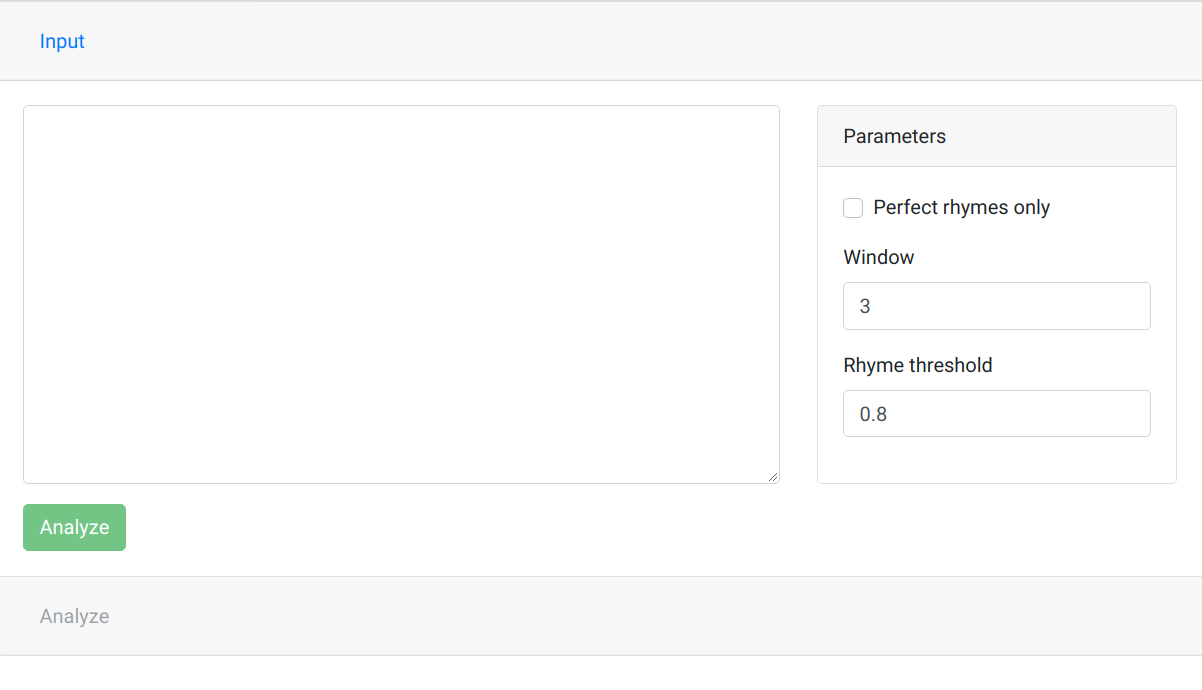
\includegraphics[scale=0.3]{../img/web-empty-form.png}
	\caption{Website's form for entering the lyrics and setting the parameters.}
	\label{web-form}
\end{figure}

\section{Visualization of the results}
Visualization page contains lyrics with scheme, matrix visualization of rhymes, and short statistics. It is primarily designed for songs of short or moderate length, longer lyrics may not fit on the screen with the analysis side-by-side, and will have to be rearranged in a column, which makes the results less comfortable to read.

\subsection{Lyrics and statistics}\label{sec-lyrics_and_stats}
Lyrics with their assigned scheme letters and line number are shown on the left, as we can see in Figure \ref{web-analysis_window5}. Rhyming lines are highlighted, each with a color corresponding to its rhyme type. For the sub-types of perfect rhyme, we selected similar colors to indicate that they are more closely related -- namely red for \textit{masculine}, orange for \textit{feminine}, and yellow for \textit{dactylic} rhymes. \textit{Imperfect} rhymes are highlighted in blue and \textit{forced} in green color. When user hovers over a rhyming line, this line and all lines rhyming with it are highlighted.

Statistics is shown on the right under the matrix. It contains song rating and percentages of different rhyme types in the song.

\begin{figure}[h]\centering
	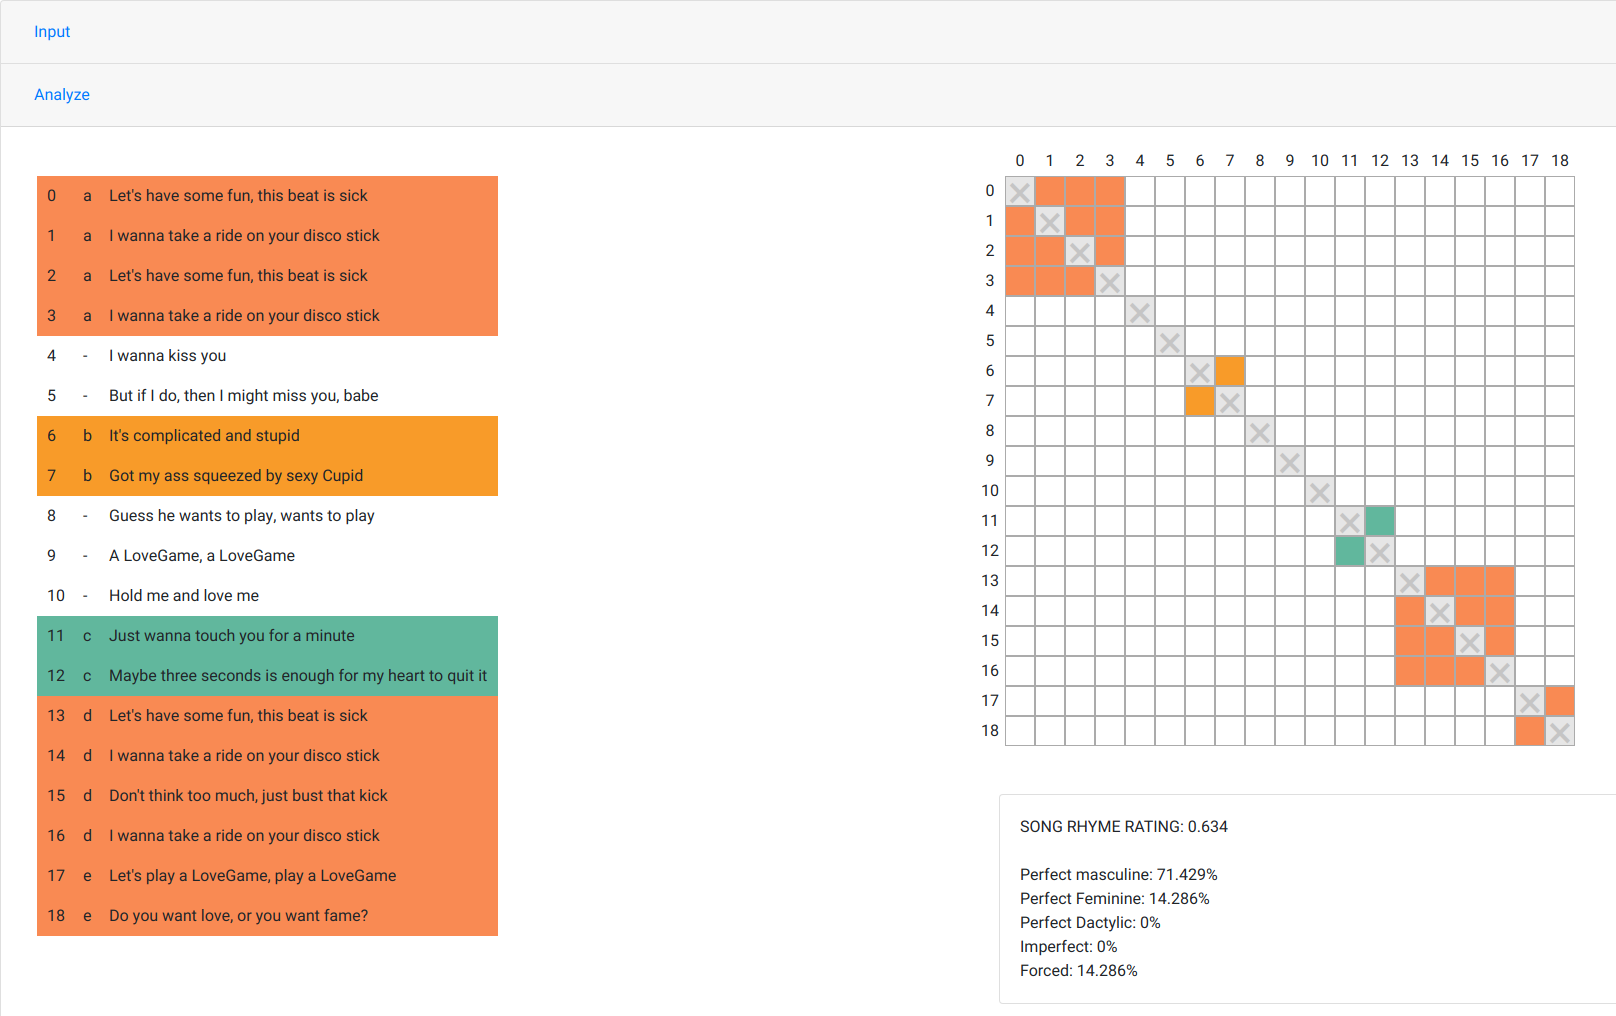
\includegraphics[scale=0.25]{../img/love_game_lady_gaga.png}
	\caption[Screenshot from analysis with default window size.]{Screenshot from analysis with default window size. Example from \textit{Love Game} by Lady Gaga.}
	\label{web-analysis_window5}
\end{figure}

\subsection{Matrix}
To make a creative visualization, we took inspiration from Colin Morris\footnote{\url{https://github.com/colinmorris}}. He came up with an idea to represent the repetitiveness of lyrics by self-similarity matrix and he demonstrated it in his project SongSim\footnote{\url{https://colinmorris.github.io/SongSim/\#/}}. In his matrix, there is one row and one column for each word of the song. For each cell, if the word in given row and column are identical, the cell is colored, otherwise it stays white (Figure \ref{songsim}).

\begin{figure}[h]\centering
	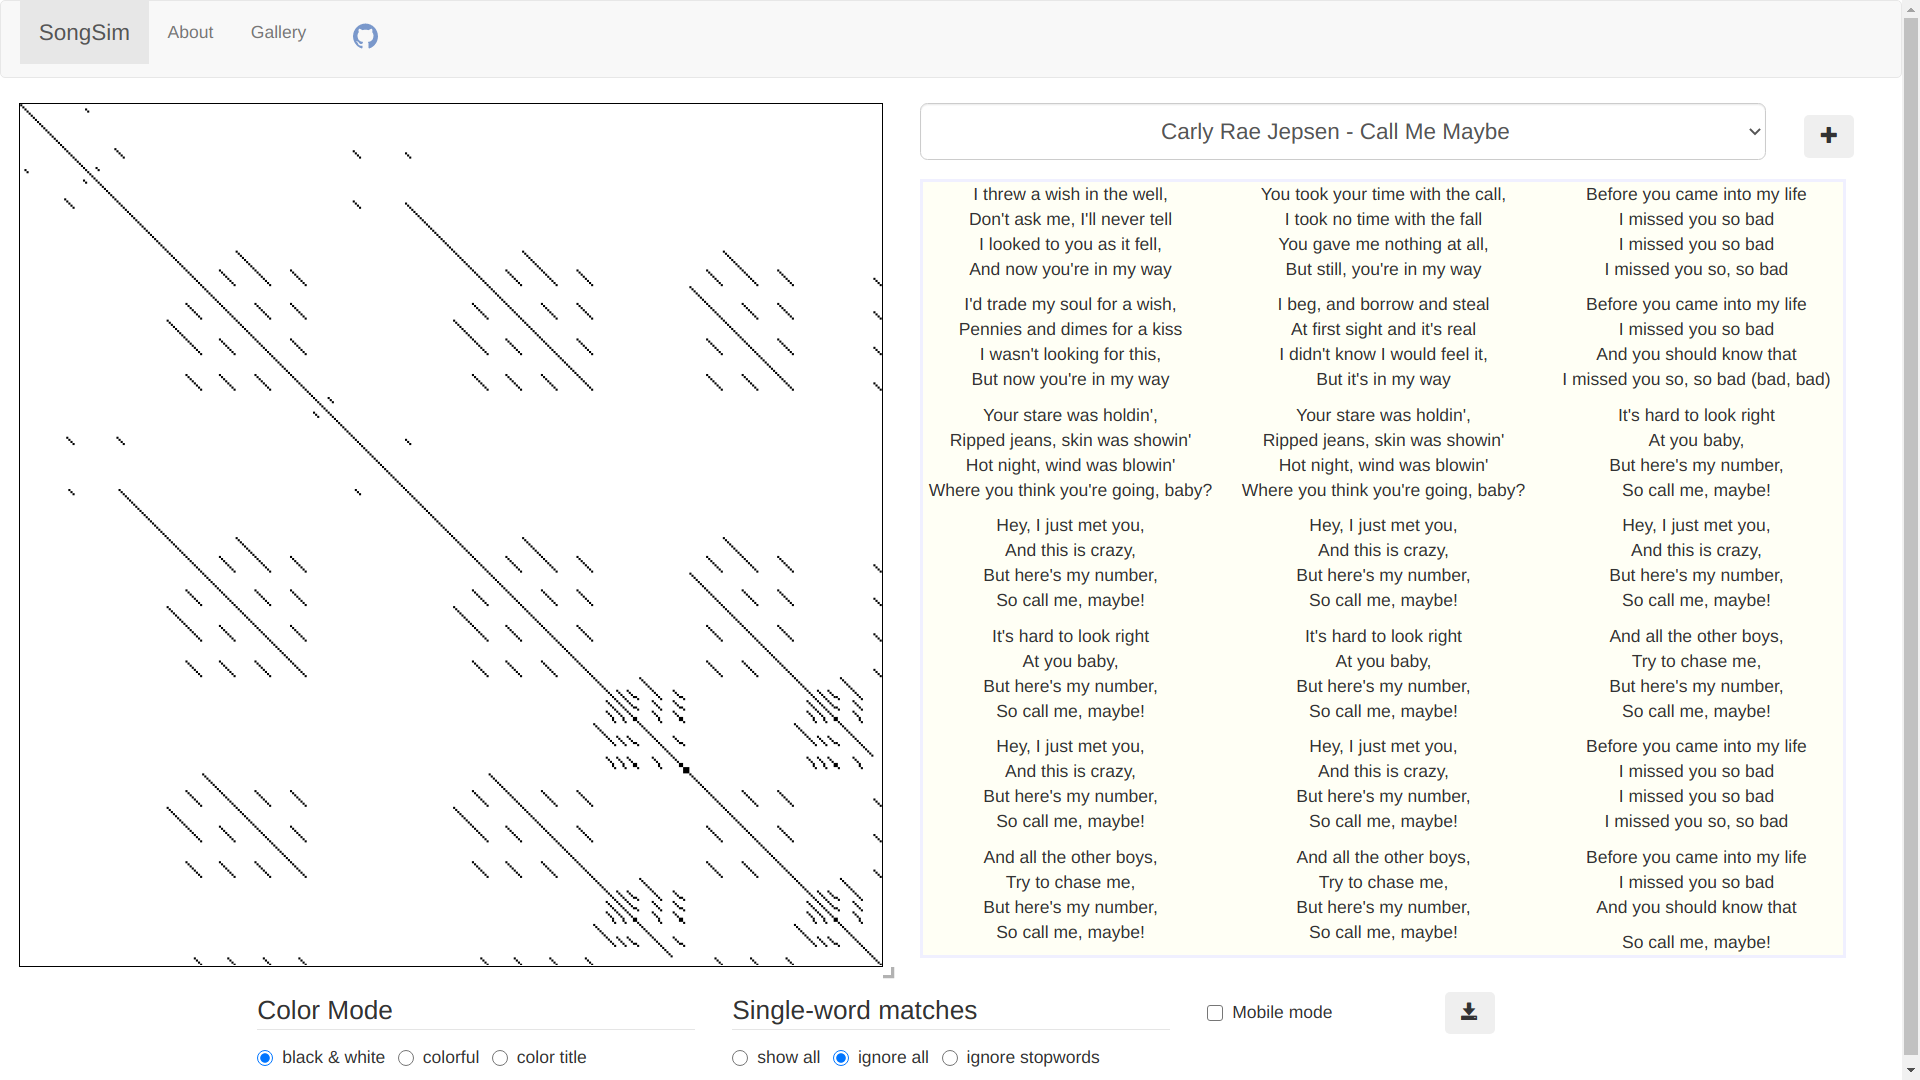
\includegraphics[scale=0.2]{../img/songsim.png}
	\caption{Screenshot of Collin's SongSim visualization of song's repetitiveness.}
	\label{songsim}
\end{figure}

Instead of words, in our matrix, we compare rhymes. For rows and columns we use rhyme scheme letters for corresponding line, and when they agree, matrix cell will receive the color of this rhyme's type, as described in section \ref{sec-lyrics_and_stats} (Figure \ref{web-analysis_window5}). For comparison with default window, in Figure \ref{web-analysis_window_all}, we include a screenshot with longer window to better demonstrate the matrix.


\begin{figure}[!h]\centering
		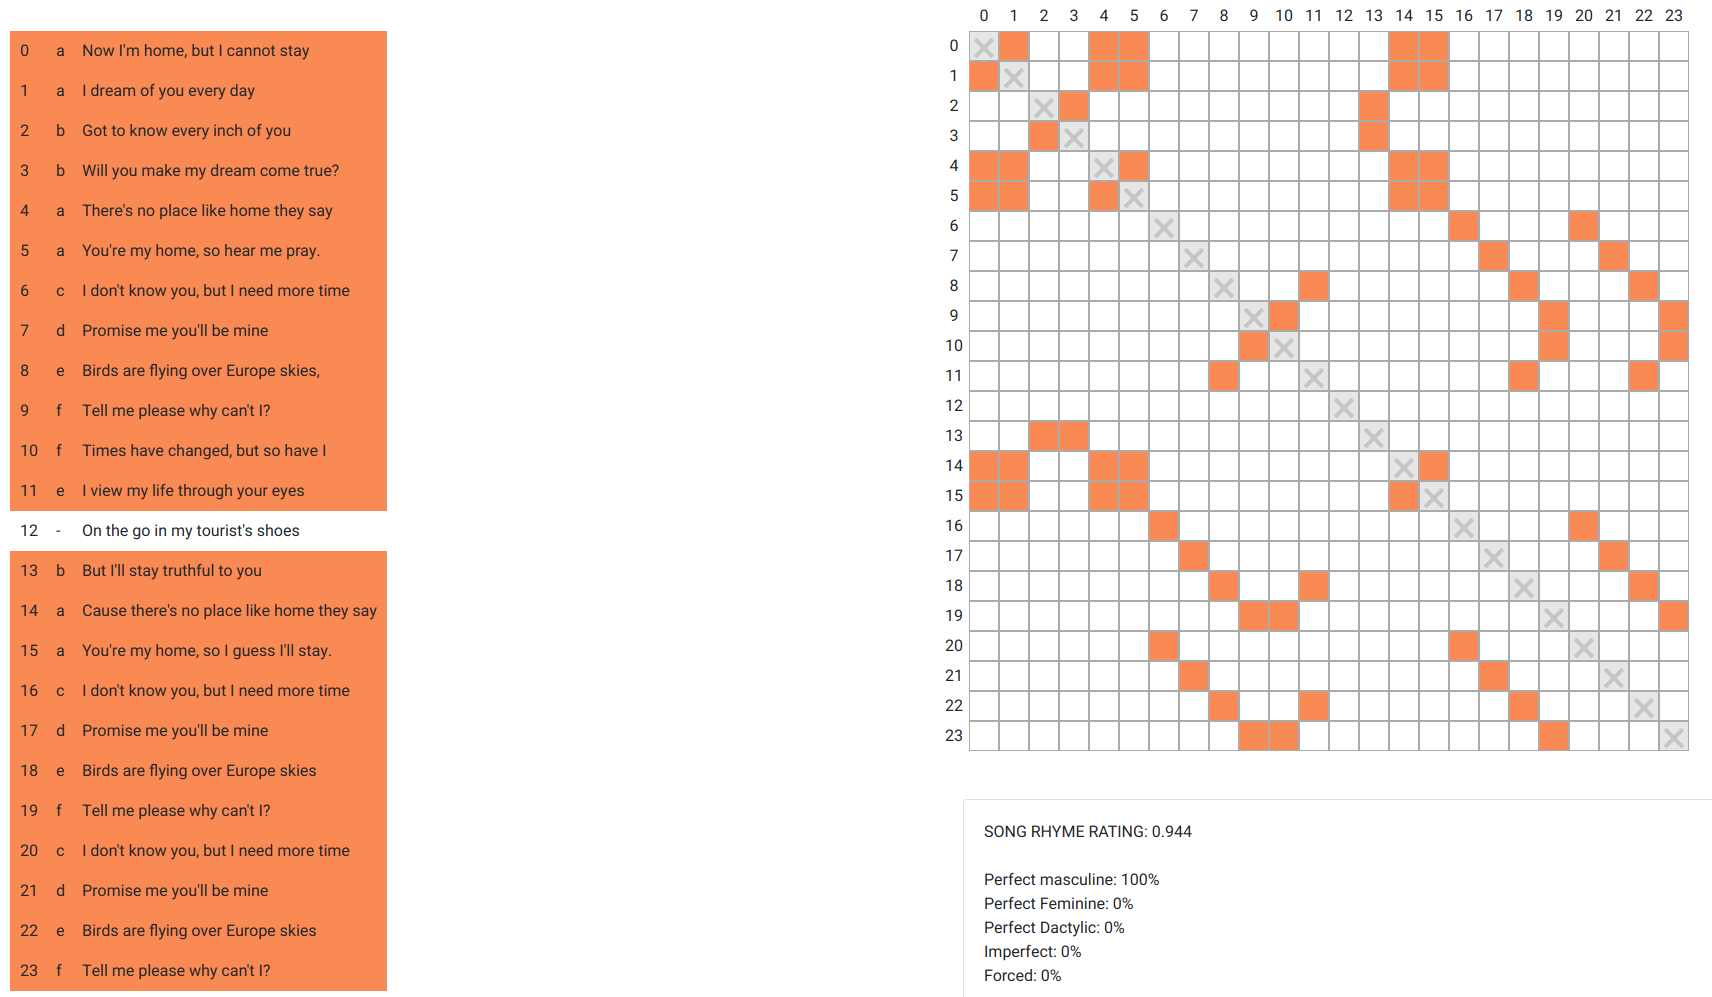
\includegraphics[scale=0.24]{../img/europes-skies.png}
	\caption[Screenshot from analysis with window size matching the song length.]{Screenshot from analysis with window size matching the song length. Example from \textit{Europe's Skies} by Alexander Rybak.}
	\label{web-analysis_window_all}
\end{figure}

So far, user has been given a large picture overview of entire song. To explore the detail, user can view rhyme's properties by hovering over the particular matrix cell. Popover will display more details as shown in Figure \ref{web-popover}. \textit{Rhyming phonemes} for both rhyming lines display only phonemes participating in rhyme -- meaning from last stressed phoneme (or where the stress was moved) onward. Lines, that correspond to this rhyme, will also be highlighted in the text on the left. 

\begin{figure}[h]\centering
		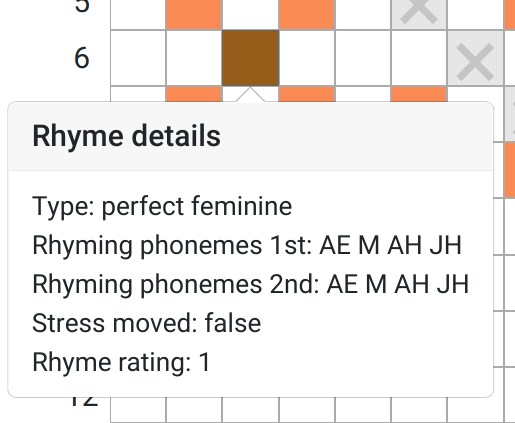
\includegraphics[scale=0.45]{../img/popover-detail.png}
	\caption{Detail of popover over one matrix tile.}
	\label{web-popover}
\end{figure}


\section{Technologies}
For the front-end of web page we used a TypeScript-based open-source web application framework --  Angular (\cite{angular}). As design library, we used Bootstrap\footnote{\url{https://getbootstrap.com/}}, and ported version of standard Bootstrap's components to Angular -- \textit{ngx-bootstrap}\footnote{\url{https://valor-software.com/ngx-bootstrap/}}. Back-end simple REST API is written in Python using micro-web framework \textit{Flask}\footnote{\url{https://flask.palletsprojects.com/en/2.0.x/}}. It calls our detector, in a classic variant without any modifications, as it was used for the evaluation in Chapter \ref{evaluation}. 

We host it at a public url \url{https://rhyme-detector.brezinovi.sk/} from our personal computer, so some short-term unavailability is possible. In case of any difficulties, please do not hesitate to contact us at \textit{patricia@brezinovi.sk}.